% Public source snapshot of the instructor's lecture notes. Numerical claims in
% this source are preserved for provenance; the chapter re-derives and checks them
% against the cited primary papers before publication.
\documentclass{article}
\usepackage{amsmath, amsfonts}
\usepackage{graphicx}
\usepackage{tikz}
\usepackage{tcolorbox}
\usepackage{booktabs}
\usepackage[dvipsnames]{xcolor}
\usepackage[margin=1in]{geometry}

\title{Lecture 11: Scaling Laws\\Predictable Paths to Better Models}
\author{Deep Learning Class}
\date{\today}

\begin{document}
\maketitle

\section{Introduction: From Architecture to Scale}

\subsection{The Thread So Far}

In our previous lectures, we have explored fundamental architectures that revolutionized deep learning:

\begin{itemize}
\item \textbf{Transformers}: Self-attention mechanism enables modeling long-range dependencies without recurrence
\item \textbf{ViT (Vision Transformers)}: Demonstrated that the same Transformer architecture works across modalities -- just change the tokenization
\item \textbf{The Scaling Thesis}: ViT showed that with enough data (JFT-300M), minimal inductive biases can outperform hand-crafted priors
\end{itemize}

This raises a crucial question: \textit{Is there a limit to this scaling approach? How far can we go by simply making models bigger and training on more data?}

The answer, discovered around 2020, is both remarkable and practical: \textbf{Performance improvements from scaling are not only possible but predictable according to mathematical laws}.

\subsection{The Central Question}

\textbf{What happens when we scale up Transformers?}

Specifically, when we increase:
\begin{enumerate}
\item \textbf{Model size} ($N$): Number of parameters
\item \textbf{Dataset size} ($D$): Number of training tokens
\item \textbf{Compute budget} ($C$): Total FLOPs used for training
\end{enumerate}

\textbf{The Discovery}: Performance (measured by cross-entropy loss $L$) improves smoothly and predictably along power-law curves. This is not just ``bigger is better'' -- it is ``bigger is better \textit{according to specific mathematical relationships}''.

\begin{tcolorbox}[colback=yellow!5!white, colframe=orange!50!black, title=Why This Matters]
Scaling laws have become the foundation of modern LLM development because they:
\begin{itemize}
\item Enable \textbf{predictive planning}: Forecast performance of expensive large models from cheaper small experiments
\item Guide \textbf{resource allocation}: Decide optimal balance between model size, data, and training compute
\item Suggest \textbf{research direction}: Indicate that scaling existing architectures is a viable path to more capable AI
\item Explain \textbf{recent progress}: Models like GPT-3, GPT-4, and others were explicitly designed using scaling law predictions
\end{itemize}
\end{tcolorbox}

This lecture connects our architectural understanding (Transformers, ViT) to the empirical science of scaling, setting the stage for understanding modern pretrained models like GPT and BERT in upcoming lectures.

\section{The Empirical Discovery: Predictable Performance}

\subsection{The Power Law Form}

Around 2020, researchers at OpenAI made a striking empirical discovery studying autoregressive language models: performance follows \textbf{power laws} \cite{kaplan2020scaling}.

\textbf{The Basic Form}:
\[
L(x) = L_{\infty} + \left(\frac{x_0}{x}\right)^{\alpha_x}
\]

where:
\begin{itemize}
\item $x$ represents the scaling factor: model size $N$, dataset size $D$, or compute $C$
\item $L$ is the test cross-entropy loss (lower is better)
\item $L_{\infty}$ is the \textbf{irreducible loss} -- the fundamental entropy of the data itself
\item The second term is the \textbf{reducible loss} -- approximately the KL divergence between the true distribution and the model
\item $x_0$ and $\alpha_x$ are constants determined empirically for each factor
\end{itemize}

\subsection{Understanding Irreducible Loss}

\textbf{What is $L_{\infty}$?}

Language (and other data modalities) has inherent ambiguity and unpredictability. Consider predicting the next word:

\begin{center}
\textit{``I went to the \underline{\hspace{2cm}}.''}
\end{center}

Multiple completions are plausible: ``store'', ``park'', ``doctor'', ``movies''. No model can predict with certainty which one the author chose. This fundamental uncertainty is $L_{\infty}$ -- the entropy of natural language itself.

\textbf{The Two-Component View}:
\begin{itemize}
\item \textbf{Irreducible loss} ($L_{\infty}$): The best possible loss achievable by any model, limited by data ambiguity
\item \textbf{Reducible loss} ($L - L_{\infty}$): The gap between the model and the optimal predictor, which decreases with scale
\end{itemize}

For language models, $L_{\infty}$ is estimated to be around 1.69 nats/token, though we can never reach it exactly \cite{kaplan2020scaling}.

\subsection{Three Scaling Dimensions}

\textbf{1. Model Size ($N$)}:
\[
L(N) = L_{\infty} + \left(\frac{N_0}{N}\right)^{\alpha_N}
\]

Typical exponent: $\alpha_N \approx 0.076$ for language models

\textbf{2. Dataset Size ($D$)}:
\[
L(D) = L_{\infty} + \left(\frac{D_0}{D}\right)^{\alpha_D}
\]

Typical exponent: $\alpha_D \approx 0.095$ for language models

\textbf{3. Compute Budget ($C$)}:
\[
L(C) = L_{\infty} + \left(\frac{C_0}{C}\right)^{\alpha_C}
\]

Typical exponent: $\alpha_C \approx 0.050$ for language models

\begin{center}
\begin{tikzpicture}[scale=1.0]
% Axes
\draw[->] (0,0) -- (10,0) node[right] {Scale (log)};
\draw[->] (0,0) -- (0,6) node[above] {Loss};

% Power law curve
\draw[thick, blue, domain=0.5:9.5] plot (\x, {0.8 + 5/\x});

% Points on curve
\foreach \x/\label in {1/10M, 2.5/100M, 4.5/1B, 6.5/10B, 8.5/100B} {
    \fill[red] (\x, {0.8 + 5/\x}) circle (3pt);
    \node[below, font=\small] at (\x, -0.2) {\label};
}

% Asymptote
\draw[dashed, gray] (0, 0.8) -- (10, 0.8) node[right, font=\small] {$L_\infty$ (irreducible)};

% Annotation
\node[align=center, font=\small] at (5, 5) {Power law: $L \approx L_\infty + (x_0/x)^{\alpha}$\\Smooth, predictable improvement};
\end{tikzpicture}
\end{center}

\textbf{Key Insight}: Smaller exponents mean slower improvement. Data scaling ($\alpha_D$) has a larger exponent than model size ($\alpha_N$), suggesting data is more efficient at reducing loss per unit increase.

\subsection{Universality Across Modalities}

Remarkably, these power laws are \textbf{not specific to language}. Henighan et al. (2020) demonstrated that the same power-law form holds across diverse domains \cite{henighan2020scaling}:

\begin{itemize}
\item Natural language (text)
\item Images (generative modeling)
\item Video
\item Multimodal text-image data
\item Mathematical problem solving
\end{itemize}

\textbf{What changes}: The specific constants ($L_{\infty}$, $x_0$, $\alpha_x$) differ by modality

\textbf{What stays the same}: The power-law functional form

This universality suggests that scaling laws reflect something fundamental about learning from data with over-parameterized neural networks, not just a quirk of language modeling.

\section{The Kaplan et al. (2020) Findings}

The seminal paper ``Scaling Laws for Neural Language Models'' \cite{kaplan2020scaling} established the foundation. Let us examine their key findings systematically.

\subsection{Key Properties of Scaling Laws}

\begin{enumerate}
\item \textbf{Hold Over Many Orders of Magnitude}
\begin{itemize}
\item Observed spanning 7+ orders of magnitude in compute
\item 6+ orders of magnitude in model size (millions to billions of parameters)
\item Remarkably consistent trends across this vast range
\end{itemize}

\item \textbf{Smooth and Continuous}
\begin{itemize}
\item No sudden jumps or phase transitions (mostly)
\item Loss decreases gradually as scale increases
\item Predictable from smaller experiments
\end{itemize}

\item \textbf{Sample Efficiency Improves with Scale}
\begin{itemize}
\item \textbf{Counterintuitive finding}: Larger models are \textit{more} sample-efficient
\item They reach a given performance level using \textit{fewer} training examples
\item Larger models learn faster per example seen
\end{itemize}

\item \textbf{Optimal Allocation Strategy}
\begin{itemize}
\item For a fixed compute budget $C$, there is an optimal allocation
\item \textbf{Kaplan et al. finding}: Most compute should go to model size
\item Specifically: $N \propto C^{0.73}$, while $D \propto C^{0.27}$ (much slower)
\item This suggested making models as large as possible
\end{itemize}

\item \textbf{Shape Independence}
\begin{itemize}
\item Performance depends strongly on scale ($N$, $D$, $C$)
\item Weak dependence on architectural details (depth vs. width, layer sizes)
\item Within reasonable limits, scale dominates over architecture
\end{itemize}
\end{enumerate}

\begin{center}
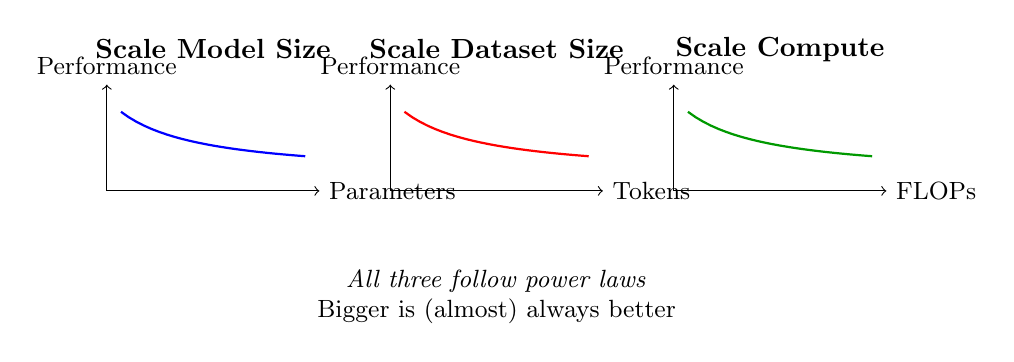
\begin{tikzpicture}[scale=0.9]
% Three subplots showing different scaling factors
\node[align=center] at (1.5, 5) {\textbf{Scale Model Size}};
\draw[->] (0,3) -- (3,3) node[right, font=\small] {Parameters};
\draw[->] (0,3) -- (0,4.5) node[above, font=\small] {Performance};
\draw[thick, blue, domain=0.2:2.8] plot (\x, {3.2 + 1.1/(1+\x)});

\node[align=center] at (5.5, 5) {\textbf{Scale Dataset Size}};
\draw[->] (4,3) -- (7,3) node[right, font=\small] {Tokens};
\draw[->] (4,3) -- (4,4.5) node[above, font=\small] {Performance};
\draw[thick, red, domain=4.2:6.8] plot (\x, {3.2 + 1.1/(1+\x-4)});

\node[align=center] at (9.5, 5) {\textbf{Scale Compute}};
\draw[->] (8,3) -- (11,3) node[right, font=\small] {FLOPs};
\draw[->] (8,3) -- (8,4.5) node[above, font=\small] {Performance};
\draw[thick, green!60!black, domain=8.2:10.8] plot (\x, {3.2 + 1.1/(1+\x-8)});

\node[align=center, font=\small] at (5.5, 1.5) {\textit{All three follow power laws}\\Bigger is (almost) always better};
\end{tikzpicture}
\end{center}

\subsection{The GPT-3 Validation}

GPT-3 (Brown et al., 2020) was a massive bet on scaling \cite{brown2020language}:

\begin{itemize}
\item \textbf{Scale}: 175 billion parameters
\item \textbf{Training compute}: $\sim$3,640 petaflop/s-days
\item \textbf{Training data}: 300 billion tokens (570 GB of text)
\item \textbf{Cost}: Estimated \$4-5 million in compute
\end{itemize}

\textbf{The remarkable outcome}: GPT-3's performance closely matched predictions from the scaling laws paper \cite{kaplan2020scaling}. This validation gave the field confidence that:
\begin{enumerate}
\item Scaling laws are reliable for planning expensive training runs
\item Simply scaling up Transformers yields substantial capability improvements
\item Investment in larger models is justified by predictable returns
\end{enumerate}

GPT-3 demonstrated emergent capabilities like few-shot learning, where the model could adapt to new tasks with just a few examples in the prompt -- a capability not explicitly trained but emerging from scale.

\section{The Chinchilla Refinement: Compute-Optimal Training}

\subsection{A Critical Re-examination}

By 2022, the field had trained several massive models following Kaplan et al.'s guidance:
\begin{itemize}
\item GPT-3: 175B parameters, 300B tokens
\item Gopher (DeepMind): 280B parameters, 300B tokens
\item Many others in the 100B+ parameter range
\end{itemize}

DeepMind researchers asked: \textit{Are we scaling optimally?}

\subsection{The Chinchilla Methodology}

To answer this rigorously, the team behind ``Training Compute-Optimal Large Language Models'' (Hoffmann et al., 2022 -- the Chinchilla paper) conducted an unprecedented systematic study \cite{hoffmann2022training}:

\textbf{Experimental Design}:
\begin{itemize}
\item Trained \textbf{over 400 models} ranging from 70M to 16B+ parameters
\item Systematically varied \textit{both} model size $N$ and training tokens $D$
\item Used multiple compute budgets from $6 \times 10^{18}$ to $3 \times 10^{21}$ FLOPs
\item Mapped the loss landscape as a function of $(N, D)$ with unprecedented precision
\end{itemize}

\textbf{Three Complementary Approaches}:

\begin{enumerate}
\item \textbf{IsoFLOP Profiles}
\begin{itemize}
\item Fix compute budget $C$
\item Train models with varying $N$ at that budget
\item Find which $N$ achieves lowest loss
\item Repeat for different budgets
\end{itemize}

\item \textbf{IsoLoss Profiles}
\begin{itemize}
\item Fix target loss value
\item Vary $N$ and measure compute needed to reach target
\item Find most efficient model size
\end{itemize}

\item \textbf{Parametric Fitting}
\begin{itemize}
\item Fit functional form to all training runs simultaneously
\item Use: $L(N, D) = E + \frac{A}{N^\alpha} + \frac{B}{D^\beta}$
\item Estimate parameters from data
\end{itemize}
\end{enumerate}

All three approaches converged on the same surprising conclusion.

\subsection{The Key Finding: Equal-Proportion Scaling}

\begin{tcolorbox}[colback=blue!5!white, colframe=blue!50!black, title=Chinchilla's Central Insight]
\textbf{For compute-optimal training}:

\[
N_{\text{opt}} \propto C^{0.5} \quad \text{and} \quad D_{\text{opt}} \propto C^{0.5}
\]

This means \textbf{parameters and tokens should scale equally}, not the parameter-heavy approach suggested by Kaplan et al.

\textbf{Practical Rule}: Approximately \textbf{20 tokens per parameter} is optimal.

\[
D_{\text{opt}} \approx 20 \times N_{\text{opt}}
\]
\end{tcolorbox}

\subsection{Parametric Form}

Chinchilla introduced a clean decomposition:

\[
L(N, D) = E + \frac{A}{N^\alpha} + \frac{B}{D^\beta}
\]

where:
\begin{itemize}
\item $E$ is the irreducible loss floor
\item First term captures model size contribution
\item Second term captures data size contribution
\item Fitted exponents: $\alpha \approx \beta \approx 0.34$
\end{itemize}

The near-equal exponents suggest \textbf{parameters and data have approximately equal importance} -- a stark contrast to Kaplan et al.'s finding that $N$ should dominate.

\subsection{Comparing the Two Approaches}

\begin{center}
\begin{tabular}{lcc}
\toprule
\textbf{Aspect} & \textbf{Kaplan et al. (2020)} & \textbf{Chinchilla (2022)} \\
\midrule
Model size scaling & $N \propto C^{0.73}$ & $N \propto C^{0.5}$ \\
Data size scaling & $D \propto C^{0.27}$ & $D \propto C^{0.5}$ \\
Strategy & Maximize $N$ & Balance $N$ and $D$ \\
Tokens per param & $\sim$2-5 & $\sim$20 \\
Example (at $10^{23}$ FLOPs) & 280B params, 300B tokens & 70B params, 1.4T tokens \\
\bottomrule
\end{tabular}
\end{center}

\subsection{The Chinchilla vs. Gopher Experiment}

DeepMind demonstrated the practical impact by training two models with the \textit{same compute budget}:

\begin{center}
\begin{tabular}{lccc}
\toprule
\textbf{Model} & \textbf{Parameters} & \textbf{Training Tokens} & \textbf{Performance} \\
\midrule
Gopher & 280B & 300B & Baseline \\
Chinchilla & 70B & 1.4T & \textbf{Better on most benchmarks} \\
\bottomrule
\end{tabular}
\end{center}

\textbf{Key Result}: The smaller Chinchilla (70B) trained on 4.7× more data outperformed the much larger Gopher (280B), using identical compute.

\begin{tcolorbox}[colback=yellow!5!white, colframe=orange!50!black, title=The Chinchilla Lesson]
\textbf{A smaller model trained on more tokens beats a larger undertrained model.}

\textbf{Previous approach} (GPT-3, Gopher):
\begin{itemize}
\item Make model as large as compute budget allows
\item Train for relatively few tokens
\item Result: Large but undertrained models
\end{itemize}

\textbf{Compute-optimal approach} (Chinchilla):
\begin{itemize}
\item Balance model size and training data
\item Train smaller model on many more tokens
\item Maintain $D \approx 20N$ ratio
\end{itemize}

\textbf{Additional benefits}:
\begin{itemize}
\item \textbf{Inference efficiency}: Smaller models are faster to run
\item \textbf{Memory requirements}: Reduced GPU memory for deployment
\item \textbf{Same training cost}: Achieved with identical FLOP budget
\end{itemize}
\end{tcolorbox}

\section{Practical Implications and Modern Models}

\subsection{The Shift in Strategy}

Chinchilla's findings fundamentally changed how the field trains large models:

\begin{center}
\begin{tabular}{lccc}
\toprule
\textbf{Model} & \textbf{Parameters} & \textbf{Training Tokens} & \textbf{Tokens/Param} \\
\midrule
GPT-3 (2020) & 175B & 300B & 1.7 \\
Gopher (2021) & 280B & 300B & 1.1 \\
\midrule
Chinchilla (2022) & 70B & 1.4T & 20.0 \\
LLaMA (2023) & 65B & 1.4T & 21.5 \\
LLaMA 2 (2023) & 70B & 2.0T & 28.6 \\
Mistral 7B (2023) & 7B & Unknown & Compute-optimal \\
\bottomrule
\end{tabular}
\end{center}

\textbf{Observation}: Post-Chinchilla models follow the 20:1 token-to-parameter ratio or exceed it.

\subsection{Compute-Optimal Projections}

Based on Chinchilla's findings, here are approximate compute-optimal configurations:

\begin{center}
\begin{tabular}{cccc}
\toprule
\textbf{Parameters} & \textbf{Optimal Tokens} & \textbf{Approx. FLOPs} & \textbf{Example} \\
\midrule
400M & 8B & $3 \times 10^{18}$ & Small research model \\
1B & 20B & $2 \times 10^{19}$ & -- \\
7B & 140B & $10^{21}$ & Mistral 7B scale \\
13B & 260B & $3 \times 10^{21}$ & LLaMA 13B scale \\
70B & 1.4T & $10^{23}$ & Chinchilla, LLaMA 65B \\
175B & 3.5T & $6 \times 10^{23}$ & Compute-optimal GPT-3 \\
500B & 10T & $5 \times 10^{24}$ & -- \\
1T & 20T & $2 \times 10^{25}$ & Hypothetical \\
\bottomrule
\end{tabular}
\end{center}

\textbf{Key Observation}: To optimally train a trillion-parameter model requires approximately 20 trillion tokens -- far exceeding available high-quality text data. This creates a \textbf{data bottleneck}.

\subsection{Compute-Optimal Training Recipe}

\begin{tcolorbox}[colback=green!5!white, colframe=green!50!black, title=Practical Recipe for Compute-Optimal Training]
\textbf{Given a fixed training budget $C$ (in FLOPs):}

\begin{enumerate}
\item \textbf{Estimate optimal model size}:
\[
N_{\text{opt}} \approx \left(\frac{C}{6 \times 20}\right)^{0.5} \text{ parameters}
\]

\item \textbf{Calculate optimal token count}:
\[
D_{\text{opt}} \approx 20 \times N_{\text{opt}} \text{ tokens}
\]

\item \textbf{Verify your budget}: Check that $C \approx 6ND$ (approximate FLOPs for Transformer training)

\item \textbf{Prioritize data quality}:
\begin{itemize}
\item High token count demands high-quality, diverse data
\item Deduplicate and filter carefully
\item Data curation is now as critical as compute
\end{itemize}

\item \textbf{Stop at compute-optimal point}:
\begin{itemize}
\item Don't train to absolute convergence
\item Stop when model reaches predicted optimal performance
\item Further training is inefficient
\end{itemize}
\end{enumerate}

\textbf{Example}: With $C = 10^{23}$ FLOPs:
\begin{align*}
N_{\text{opt}} &\approx 70\text{B parameters} \\
D_{\text{opt}} &\approx 1.4\text{T tokens}
\end{align*}

This is Chinchilla's configuration, which outperformed Gopher's 280B parameters at the same compute.
\end{tcolorbox}

\section{Understanding Why Scaling Works}

\subsection{What Do Scaling Laws Actually Measure?}

Scaling laws measure \textbf{cross-entropy loss} on held-out test data. But what does this mean practically?

\textbf{Cross-entropy loss} quantifies how well the model's predicted probability distribution matches the true distribution:
\[
L = -\mathbb{E}_{x \sim \text{data}}[\log P_{\text{model}}(x)]
\]

\textbf{Lower loss means}:
\begin{itemize}
\item Better next-token predictions
\item More accurate probability estimates
\item Closer match to human language patterns
\end{itemize}

\textbf{Connection to capabilities}: While scaling laws predict loss, they don't directly predict which specific capabilities emerge. However, better next-token prediction enables:
\begin{itemize}
\item Coherent long-form generation
\item Following instructions
\item Few-shot learning (learning from examples in context)
\item Reasoning through complex problems
\item Factual knowledge retrieval
\end{itemize}

\subsection{Why Power Laws?}

\textbf{The mystery}: Why do such simple power-law relationships govern complex neural network training?

\textbf{Theoretical perspectives}:

\begin{enumerate}
\item \textbf{Intrinsic Dimension Hypothesis}
\begin{itemize}
\item Natural data (text, images) lives on a low-dimensional manifold
\item Models learn the shape of this manifold
\item More parameters or data allow resolving the manifold at finer scale
\item Geometric arguments suggest error scales as $N^{-c/d}$ where $d$ is intrinsic dimension
\end{itemize}

\item \textbf{Effective Model Complexity}
\begin{itemize}
\item Not all parameters are equally ``useful''
\item Effective number of useful parameters grows sub-linearly
\item Over-parameterization provides flexibility without overfitting
\end{itemize}

\item \textbf{Optimization Dynamics}
\begin{itemize}
\item Gradient descent naturally finds solutions with certain complexity
\item Larger models can represent finer-grained patterns
\item Power laws reflect the learning dynamics of SGD
\end{itemize}
\end{enumerate}

\textbf{Current status}: Theory is developing but incomplete. The empirical power laws work remarkably well, even though we don't fully understand why.

\subsection{Sample Efficiency: A Surprising Finding}

One of the most counterintuitive discoveries: \textbf{larger models are more sample-efficient}.

\begin{center}
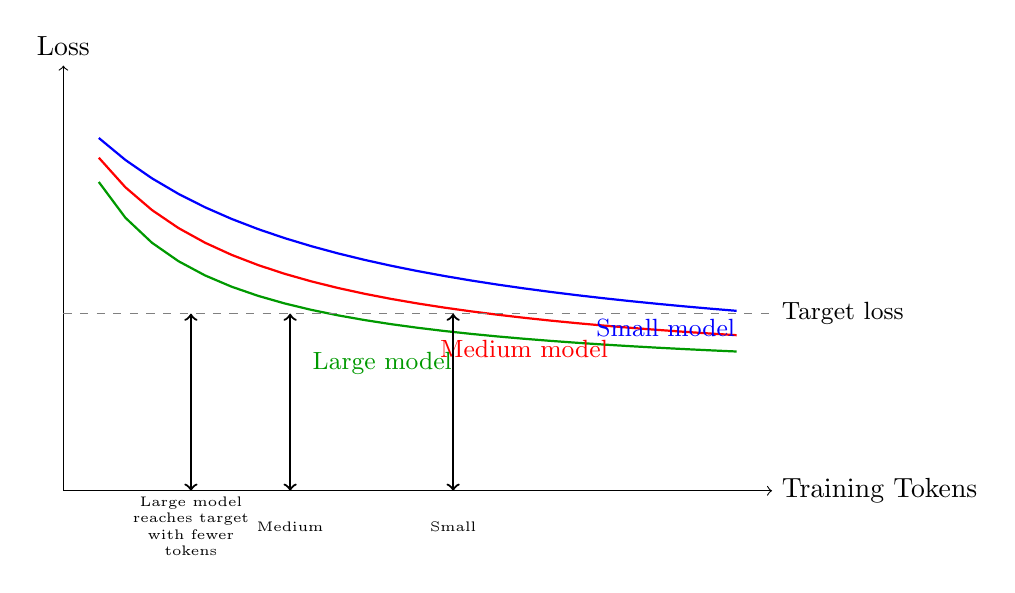
\begin{tikzpicture}[scale=0.9]
\draw[->] (0,0) -- (10,0) node[right] {Training Tokens};
\draw[->] (0,0) -- (0,6) node[above] {Loss};

% Three curves for different model sizes
\draw[thick, blue, domain=0.5:9.5] plot (\x, {1.5 + 4/(1+0.3*\x)});
\draw[thick, red, domain=0.5:9.5] plot (\x, {1.5 + 4/(1+0.5*\x)});
\draw[thick, green!60!black, domain=0.5:9.5] plot (\x, {1.5 + 4/(1+0.8*\x)});

% Labels
\node[blue, font=\small] at (8.5, 2.3) {Small model};
\node[red, font=\small] at (6.5, 2.0) {Medium model};
\node[green!60!black, font=\small] at (4.5, 1.8) {Large model};

% Horizontal line showing target loss
\draw[dashed, gray] (0, 2.5) -- (10, 2.5);
\node[right, font=\small] at (10, 2.5) {Target loss};

% Arrows showing fewer samples needed
\draw[<->, thick] (1.8, 0) -- (1.8, 2.5);
\node[font=\tiny, align=center] at (1.8, -0.5) {Large model\\reaches target\\with fewer\\tokens};

\draw[<->, thick] (3.2, 0) -- (3.2, 2.5);
\node[font=\tiny, align=center] at (3.2, -0.5) {Medium};

\draw[<->, thick] (5.5, 0) -- (5.5, 2.5);
\node[font=\tiny, align=center] at (5.5, -0.5) {Small};
\end{tikzpicture}
\end{center}

\textbf{Interpretation}:
\begin{itemize}
\item Larger models extract more information per training example
\item They converge faster (in terms of data seen)
\item This is why scaling model size is efficient, not wasteful
\end{itemize}

This finding justified the initial push toward larger models, though Chinchilla showed data shouldn't be neglected.

\section{Why Scaling Laws Matter for Modern AI}

\subsection{Predictive Power}

Scaling laws enable \textbf{forward planning} for expensive training runs:

\begin{enumerate}
\item \textbf{Performance forecasting}:
\begin{itemize}
\item Train small models (cheap)
\item Fit power-law curves
\item Extrapolate to predict large model performance
\item Decide if training cost is justified
\end{itemize}

\item \textbf{Resource allocation}:
\begin{itemize}
\item Given compute budget, determine optimal $N$ and $D$
\item Avoid wasting resources on suboptimal configurations
\item Balance infrastructure decisions (GPUs, data storage, etc.)
\end{itemize}

\item \textbf{Risk management}:
\begin{itemize}
\item Validate predictions with intermediate checkpoints
\item Catch issues early before full training
\item OpenAI explicitly used this for GPT-4
\end{itemize}
\end{enumerate}

\subsection{The GPT-4 Success Story}

OpenAI's technical report for GPT-4 (2023) explicitly states:

\begin{quote}
\textit{``We developed infrastructure and optimization methods that have very predictable behavior across multiple scales. This allowed us to accurately predict aspects of the performance of GPT-4 from models trained using the same methodology but using 1,000× -- 10,000× less compute than GPT-4.''}
\end{quote}

This demonstrates the practical value of scaling laws for planning multi-million dollar training runs.

\subsection{Democratization Through Compute-Optimal Training}

Chinchilla's findings have \textbf{democratizing effects}:

\begin{itemize}
\item \textbf{Smaller organizations can compete}: A 7B compute-optimal model can match a 30B undertrained model
\item \textbf{Faster inference}: Smaller models are more practical to deploy
\item \textbf{Lower barriers}: Less GPU memory and bandwidth needed
\item \textbf{Open-source models}: LLaMA, Mistral, and others leverage compute-optimal training
\end{itemize}

The shift from ``bigger is better'' to ``compute-optimal is better'' has enabled a flourishing ecosystem of capable open models.

\section{Limits, Caveats, and Future Directions}

\subsection{Where Scaling Laws Break Down}

\begin{tcolorbox}[colback=red!5!white, colframe=red!75!black, title=Warning: Scaling Laws Have Limits]
Scaling laws are \textbf{empirical observations}, not fundamental physics:

\begin{enumerate}
\item \textbf{Irreducible Loss is Real}
\begin{itemize}
\item Performance \textit{must} plateau at $L_{\infty}$
\item Language has inherent ambiguity and unpredictability
\item We cannot predict perfectly if multiple continuations are valid
\item For language: $L_{\infty} \approx 1.69$ nats/token (estimated)
\end{itemize}

\item \textbf{Possible Breakdown at Extreme Scales}
\begin{itemize}
\item Laws have held up to GPT-4 scale
\item But might break down at even larger scales
\item Inconsistencies between $L(C)$ and $L(D)$ suggest potential issues
\item Phase transitions or discontinuities are possible
\end{itemize}

\item \textbf{Emergence is Unpredictable}
\begin{itemize}
\item Scaling laws predict \textit{loss reduction}
\item They don't predict \textit{which} capabilities emerge
\item They don't predict \textit{when} capabilities emerge
\item Qualitative behavioral changes remain surprising
\end{itemize}

\item \textbf{Inference Costs Scale Linearly}
\begin{itemize}
\item Training follows power laws
\item But using the model scales linearly with size
\item Bigger models are slower and more expensive to run
\item This creates practical deployment constraints
\end{itemize}

\item \textbf{Data Quality is Critical}
\begin{itemize}
\item Scaling laws assume high-quality, diverse data
\item Low-quality or narrow data reduces gains
\item Data contamination and duplication hurt performance
\item Bias in training data amplifies at scale
\end{itemize}
\end{enumerate}
\end{tcolorbox}

\subsection{The Data Bottleneck}

Chinchilla's finding that $D_{\text{opt}} \approx 20N$ creates a new challenge:

\begin{center}
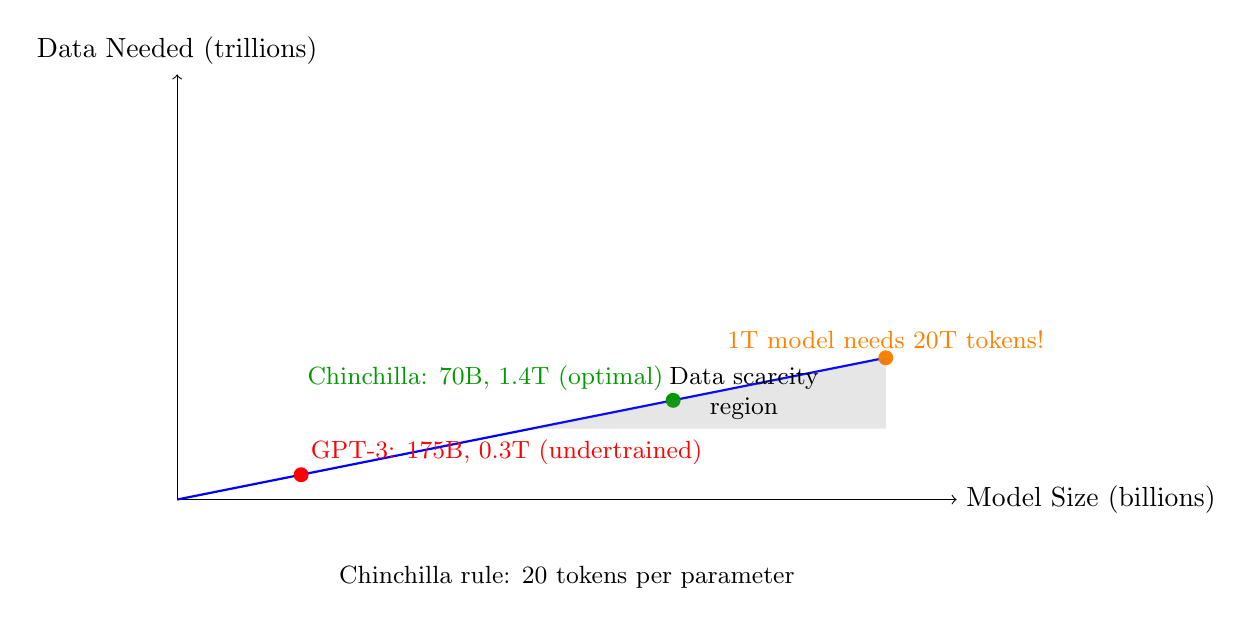
\begin{tikzpicture}[scale=0.9]
\draw[->] (0,0) -- (11,0) node[right] {Model Size (billions)};
\draw[->] (0,0) -- (0,6) node[above] {Data Needed (trillions)};

% Linear relationship D = 20N
\draw[thick, blue, domain=0:10] plot (\x, {0.2*\x});

% Points for different models
\fill[red] (1.75, 0.35) circle (3pt) node[above right, font=\small] {GPT-3: 175B, 0.3T (undertrained)};
\fill[green!60!black] (7, 1.4) circle (3pt) node[above left, font=\small] {Chinchilla: 70B, 1.4T (optimal)};
\fill[orange] (10, 2) circle (3pt) node[above, font=\small] {1T model needs 20T tokens!};

% Shaded region showing data scarcity
\fill[gray, opacity=0.2] (5, 1) -- (10, 1) -- (10, 2) -- (5, 1);
\node[align=center, font=\small] at (8, 1.5) {Data scarcity\\region};

\node[below, font=\small] at (5.5, -0.8) {Chinchilla rule: 20 tokens per parameter};
\end{tikzpicture}
\end{center}

\textbf{The problem}: High-quality text data is finite. Estimates suggest:
\begin{itemize}
\item Total internet text: $\sim$10-50 trillion tokens
\item High-quality filtered text: $\sim$1-5 trillion tokens
\item Already used for LLaMA, GPT-4, etc.
\end{itemize}

\textbf{Implications}: To optimally train a 500B+ parameter model requires 10T+ tokens -- approaching the limits of available data.

\subsection{Beyond the Data Wall}

The data bottleneck is driving new research directions:

\begin{enumerate}
\item \textbf{Synthetic Data Generation}
\begin{itemize}
\item Use models to generate training data
\item Self-improvement loops
\item Risk of model collapse if done naively
\end{itemize}

\item \textbf{Data Augmentation}
\begin{itemize}
\item Paraphrasing and variation
\item Back-translation
\item Instruction-following data from templates
\end{itemize}

\item \textbf{Multimodal Learning}
\begin{itemize}
\item Images, video, audio as additional modalities
\item Cross-modal knowledge transfer
\item Web-scale multimodal data (LAION-5B, etc.)
\end{itemize}

\item \textbf{Improved Data Efficiency}
\begin{itemize}
\item Better tokenization (fewer tokens per concept)
\item Curriculum learning (train on easy then hard data)
\item Active learning (select most informative examples)
\end{itemize}

\item \textbf{Retrieval-Augmented Models}
\begin{itemize}
\item Retrieve from external knowledge bases
\item Don't memorize everything in parameters
\item Reduce parameter count requirements
\end{itemize}
\end{enumerate}

\subsection{Architecture and Algorithms Still Matter}

While scale dominates, improvements in architecture and training remain valuable:

\begin{itemize}
\item \textbf{Sparse models}: Mixture-of-Experts (MoE) architectures increase capacity without proportional compute
\item \textbf{Efficient attention}: Flash Attention, sparse attention patterns reduce memory and compute
\item \textbf{Better optimization}: Improved learning rate schedules, normalization, initialization
\item \textbf{Data curation}: Better filtering, deduplication, and quality control improve sample efficiency
\end{itemize}

These improvements affect the \textit{constants} in scaling laws, making training more efficient even if the power-law form persists.

\subsection{Theoretical Understanding}

\textbf{Open questions}:
\begin{itemize}
\item Why do power laws emerge from gradient descent?
\item What determines the specific exponents $\alpha_x$?
\item Can we derive scaling laws from first principles?
\item What is the true irreducible loss for language?
\end{itemize}

\textbf{Current theories}:
\begin{itemize}
\item Connection to manifold dimension of data
\item Neural tangent kernel analysis
\item Statistical learning theory bounds
\item Information-theoretic perspectives
\end{itemize}

The field is actively working to build theoretical foundations for these empirical observations.

\section{Connection to Next Lectures}

\subsection{Setting the Stage for GPT and BERT}

Scaling laws explain \textit{why} the models we study next are so effective:

\begin{itemize}
\item \textbf{GPT (Generative Pre-trained Transformer)}:
\begin{itemize}
\item Autoregressive language model (predicts next token)
\item Directly optimizes the objective measured by scaling laws
\item Scaling from GPT-1 to GPT-4 follows predicted improvements
\end{itemize}

\item \textbf{BERT (Bidirectional Encoder Representations from Transformers)}:
\begin{itemize}
\item Masked language modeling (predict hidden tokens)
\item Different objective but similar scaling behavior
\item Demonstrates scaling laws apply to encoder-only models too
\end{itemize}
\end{itemize}

\subsection{The Pretraining Paradigm}

Scaling laws justify the now-dominant paradigm:

\begin{enumerate}
\item \textbf{Pretraining}:
\begin{itemize}
\item Train large model on massive unlabeled data
\item Scale according to compute-optimal principles
\item Learn general language representations
\end{itemize}

\item \textbf{Fine-tuning}:
\begin{itemize}
\item Adapt pretrained model to specific tasks
\item Requires orders of magnitude less data and compute
\item Leverages knowledge from pretraining
\end{itemize}
\end{enumerate}

This two-stage approach is enabled by scaling laws showing that large pretrained models generalize well.

\subsection{Looking Ahead}

In upcoming lectures, we will study:

\begin{itemize}
\item \textbf{GPT family}: How autoregressive pretraining at scale creates few-shot learners
\item \textbf{BERT family}: How masked language modeling creates powerful encoders
\item \textbf{Fine-tuning strategies}: How to adapt large pretrained models efficiently
\item \textbf{Instruction following}: How models learn to follow human instructions
\end{itemize}

Understanding scaling laws provides the foundation for appreciating why these models work and how to train them effectively.

\section{Key Takeaways}

\begin{enumerate}
\item \textbf{Scaling laws are empirical power laws} describing how loss decreases with model size, data size, and compute

\item \textbf{Kaplan et al. (2020)} established that performance improves smoothly and predictably over many orders of magnitude

\item \textbf{Chinchilla (2022)} refined the optimal allocation: parameters and tokens should scale equally ($D \approx 20N$)

\item \textbf{Compute-optimal training} produces better and more efficient models than simply maximizing parameters

\item \textbf{Data quality and quantity} are now as critical as compute -- the field faces a data bottleneck

\item \textbf{Scaling laws enable prediction}, guiding multi-million dollar decisions on model training

\item \textbf{Universal across modalities}: Similar power laws hold for language, vision, and other domains

\item \textbf{Limits exist}: Irreducible loss, data scarcity, and inference costs constrain pure scaling approaches

\item \textbf{Architecture and algorithms matter} for improving the constants in scaling laws

\item \textbf{Foundation for modern AI}: Scaling laws justify and guide the pretrain-then-finetune paradigm
\end{enumerate}

\section*{References}

\begin{thebibliography}{99}

\bibitem{kaplan2020scaling}
Kaplan, J., McCandlish, S., Henighan, T., Brown, T.B., Chess, B., Child, R., Gray, S., Radford, A., Wu, J., and Amodei, D. (2020).
\textit{Scaling laws for neural language models}.
arXiv preprint arXiv:2001.08361.

\bibitem{brown2020language}
Brown, T., Mann, B., Ryder, N., Subbiah, M., Kaplan, J.D., Dhariwal, P., Neelakantan, A., Shyam, P., Sastry, G., Askell, A., et al. (2020).
\textit{Language models are few-shot learners}.
Advances in Neural Information Processing Systems, 33:1877--1901.

\bibitem{henighan2020scaling}
Henighan, T., Kaplan, J., Katz, M., Chen, M., Hesse, C., Jackson, J., Jun, H., Brown, T.B., Dhariwal, P., Gray, S., et al. (2020).
\textit{Scaling laws for autoregressive generative modeling}.
arXiv preprint arXiv:2010.14701.

\bibitem{hoffmann2022training}
Hoffmann, Jordan and Borgeaud, Sebastian and Mensch, Arthur and Buchatskaya, Elena and Cai, Trevor and Rutherford, Eliza and Casas, Diego de Las and Hendricks, Lisa Anne and Welbl, Johannes and Clark, Aidan and others (2022).
\textit{Training compute-optimal large language models}.
arXiv preprint arXiv:2203.15556.

\end{thebibliography}

\end{document}
